\subsection{Idealized biogeochemical model : NChlPZD, N$2$ChlPZD$2$, N$2$P$2$Z$2$D$2$}
ROMSTOOLS can help for the design of ROMS biogeochemical
experiments. For the initial conditions and lateral boundary
conditions, WOA provides a seasonal climatology for nitrateD
concentration and WOA or SeaWifs can be used to obtain a 
seasonal climatology of surface chlorophyll concentration.
Phytoplankton is estimated by a constant chlorophyll/phytoplankton 
ratio derived from previous simulations. Zooplankton is estimated
in a similar way. The part which should be edited by the user in 
romstools\_param.m is:\\
\\ 
\%\%\%\%\%\%\%\%\%\%\%\%\%\%\%\%\%\%\%\%\%\%\%\%\%\%\%\%\%\%\%\\
\%\\
\% Open boundaries and initial conditions parameters\\
\%   used by make\_clim.m, make\_biol.m, make\_bry.m\\
\%\%\%\%\%\%\%\%\%\%\%\%\%\%\%\%\%\%\%\%\%\%\%\%\%\%\%\%\%\%\%\\
\%\\
\% World Ocean Atlas directory (WOA2001 or WOA2005) \\
\%\\
woa\_dir=[ROMSTOOLS\_dir,'WOA2005/'];\\
\%\\
\% Surface chlorophyll seasonal climatology (WOA2001 or SeaWifs)\\
\%\\
chla\_dir=[ROMSTOOLS\_dir,'SeaWifs/'];\\
\%\\\\
Variables description :
\begin{itemize}
\item woa\_dir=[ROMSTOOLS\_dir,'WOA2005/'] : Directory where the World Ocean
Atlas 2005 climatology \citep{Con02} is located. The World Ocean
Atlas 2001 climatology can also be used.
\item chla\_dir=[ROMSTOOLS\_dir,'SeaWifs/'] : Directory of the surface 
chlorophyll seasonal climatology.
\end{itemize}
Run make\_biol in the Matlab session :\\
$>>$\\
$>>$ make\_biol\\\\
You should obtain :\\
-------------------------------------------------------------------------------\\
Add\_no3: creating variables and attributes for the OA file\\
Add\_no3: creating variables and attributes for the Climatology file\\
\\ 
 Ext tracers: Roa = 0 km - default value = NaN\\
 Ext tracers: horizontal interpolation of the annual data\\
 Ext tracers: horizontal interpolation of the seasonal data\\
time index: 1 of total: 4\\
time index: 2 of total: 4\\
time index: 3 of total: 4\\
time index: 4 of total: 4\\
 \\
 Vertical interpolations\\
 \\
 NO3...\\
 Time index: 1 of total: 4\\
 Time index: 2 of total: 4\\
 Time index: 3 of total: 4\\
 Time index: 4 of total: 4\\
 \\
 CHla...\\
Add\_chla: creating variable and attribute\\
...\\
Make a few plots...\\
-------------------------------------------------------------------------------\\\\
The cpp keys related to these biology models are :
\begin{itemize}
\item BIO\_NChlPZD : Select a 5 components (Nitrate, Chlorophyll, Phytoplankton, 
Zooplankton, Detritus) biogeochemical model.
\item BIO\_N2ChlPZD2 : Select a 7 components (Nitrate, Ammonium, Chlorophyll, 
Phytoplankton, Zooplankton, Small Detritus, Large Detritus) biogeochemical model. 
\item BIO\_N2P2Z2D2 : Select a 8 components (Nitrate, Ammonium, Small  
Phytoplankton, Large Phytoplankton, Small Zooplankton, Large Zooplankton,
Small Detritus, Large Detritus) biogeochemical model. 
\item DIAGNOSTICS\_BIO : Define if writing out fluxes between the biological
components.\\
\end{itemize}


\subsection{PISCES biogeochemical model}
This latter is a more complex biogeochemical model, firstly coupled to OPA and now a
beta version of the model can be coupled with ROMS\_AGRIF. It is nicely
described in \citep{AumontNoticePisces05} provide in the documentation section of
ROMS\_TOOLS.\\ \\
The cpp keys related to this biogeochemical model are :
\begin{itemize}
\item PISCES : Select the PISCES biogeochemical model
\item DIAGNOSTICS\_BIO : Define if writing out fluxes between the biological
components. \\
\end{itemize}
ROMS\_TOOLS provides preprocessing tools to design experiment using this
biogeochemical model : make\_ini\_pisces, make\_clim\_pisces, make\_bry\_pisces,
make\_bio\_forcing.m as for the climatological experiments.\footnote{These routines
  use add\_dic.m, add\_doc.m, add\_fer.m, add\_o2.m, add\_talk.m, add\_sio3.m,
  add\_ini\_dic.m, add\_ini\_doc.m, add\_ini\_fer.m, add\_ini\_o2.m,
  add\_ini\_talk.m, add\_ini\_po4.m, add\_ini\_sio3.m}. This part of ROMS\_TOOLS use
the World Ocean Atlas, called WOAPISCES in ROMS\_TOOLS, that provides the global data
of Iron (Fe), Silicate (SiO3), Oxygen (O2), Phosphate (PO4)) dic (dissolved organic
carbon), doc (dissolved inorganic carbon) and Alkanility. \\

\noindent In the make\_clim\_pisces :
\\
\%\%\%\%\%\%\%\%\%\%\%\%USERS DEFINED VARIABLES\%\%\%\%\%\%\%\%\\\
\%\\
\%  Switches for selecting what to process ($1$=$ON$)\\
\%\\
romstools\_param\\
\%\\
\% Climatology files\\
\%\\
\textbf{DATADIR='../Data\_Roms\_Local/';}\\
no3\_seas\_data  = [DATADIR,'WOAPISCES/no3\_seas.cdf'];\\
no3\_ann\_data   = [DATADIR,'WOAPISCES/no3\_ann.cdf'];\\
po4\_seas\_data  = [DATADIR,'WOAPISCES/po4\_seas.cdf'];\\
po4\_ann\_data   = [DATADIR,'WOAPISCES/po4\_ann.cdf'];\\
o2\_seas\_data   = [DATADIR,'WOAPISCES/o2\_seas.cdf'];\\
o2\_ann\_data    = [DATADIR,'WOAPISCES/o2\_ann.cdf'];\\
sio3\_seas\_data = [DATADIR,'WOAPISCES/sio3\_seas.cdf'];\\
sio3\_ann\_data  = [DATADIR,'WOAPISCES/sio3\_ann.cdf'];\\
dic\_seas\_data  = [DATADIR,'WOAPISCES/dic\_seas.cdf'];\\
dic\_ann\_data   = [DATADIR,'WOAPISCES/dic\_ann.cdf'];\\
talk\_seas\_data = [DATADIR,'WOAPISCES/talk\_seas.cdf'];\\
talk\_ann\_data  = [DATADIR,'WOAPISCES/talk\_ann.cdf'];\\
doc\_seas\_data  = [DATADIR,'WOAPISCES/doc\_seas.cdf'];\\
doc\_ann\_data   = [DATADIR,'WOAPISCES/doc\_ann.cdf'];\\
fer\_seas\_data  = [DATADIR,'WOAPISCES/fer\_seas.cdf'];\\
fer\_ann\_data   = [DATADIR,'WOAPISCES/fer\_ann.cdf'];\\
dust\_seas\_data = [DATADIR,'WOAPISCES/dust\_seas.cdf'];\\
dust\_ann\_data  = [DATADIR,'WOAPISCES/dust\_ann.cdf'];\\
\%\\
cycle=woa\_cycle;\\
NO3min=1;\\


\noindent To add the boundary condition for the PISCES variables in xxx\_clm.nc file : \\
$>>$\\
$>>$ make\_clim\_pisces\\

Add\_no3: creating variables and attributes for the OA file\\
write no3time\\
Add\_po4: creating variables and attributes for the OA file\\
Add\_sio3: creating variables and attributes for the OA file\\
Add\_o2: creating variables and attributes for the OA file\\
Add\_dic: creating variables and attributes for the OA file\\
Add\_talk: creating variables and attributes for the OA file\\
Add\_doc: creating variables and attributes for the OA file\\
Add\_fer: creating variables and attributes for the OA file\\
 \\
 Ext tracers: Roa = 0 km - default value = NaN\\
 Ext tracers: horizontal interpolation of the seasonal data\\
time index: 1 of total: 12\\
time index: 2 of total: 12\\
time index: 3 of total: 12\\
time index: 4 of total: 12\\
time index: 5 of total: 12\\
time index: 6 of total: 12\\
time index: 7 of total: 12\\
time index: 8 of total: 12\\
time index: 9 of total: 12\\
time index: 10 of total: 12\\
time index: 11 of total: 12\\
time index: 12 of total: 12\\

\newpage
\noindent To add initial condition for PISCES variables to xxx\_ini.nc file : \\
$>>$\\
$>>$ make\_ini\_pisces\\

\begin{figure}[!htbp]
\subfigure[Surface map]{
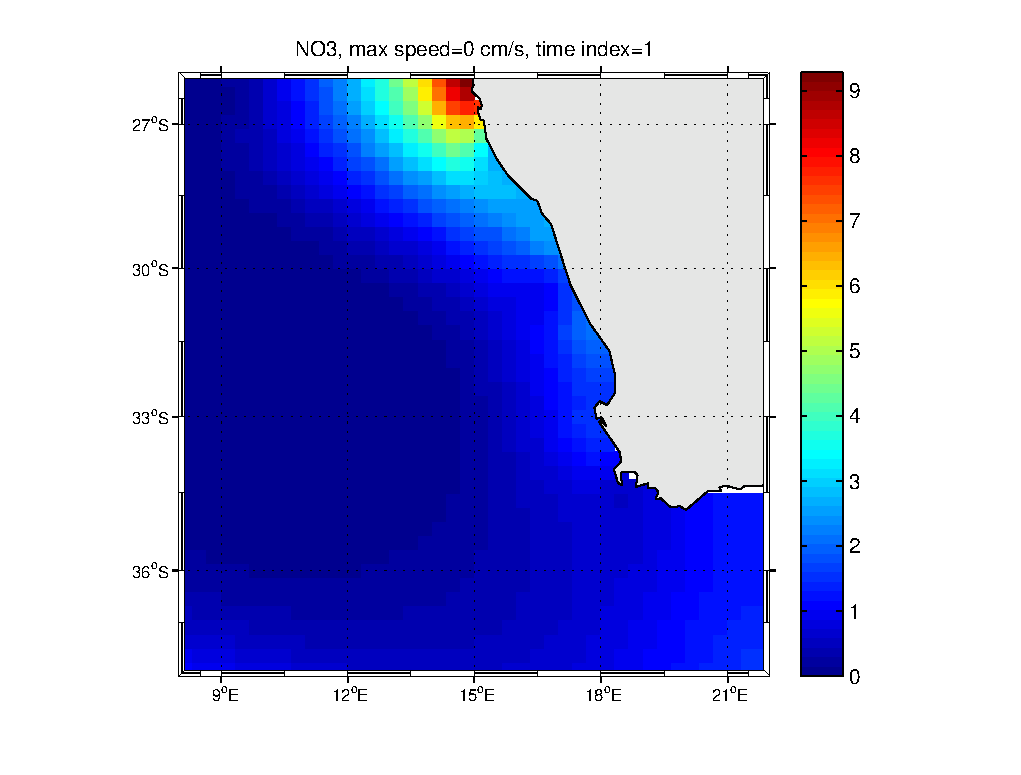
\includegraphics[width=0.4\textwidth]{NO3_surf_t1.eps}}%
\hfill
\subfigure[vertical sections along open boundaries]{
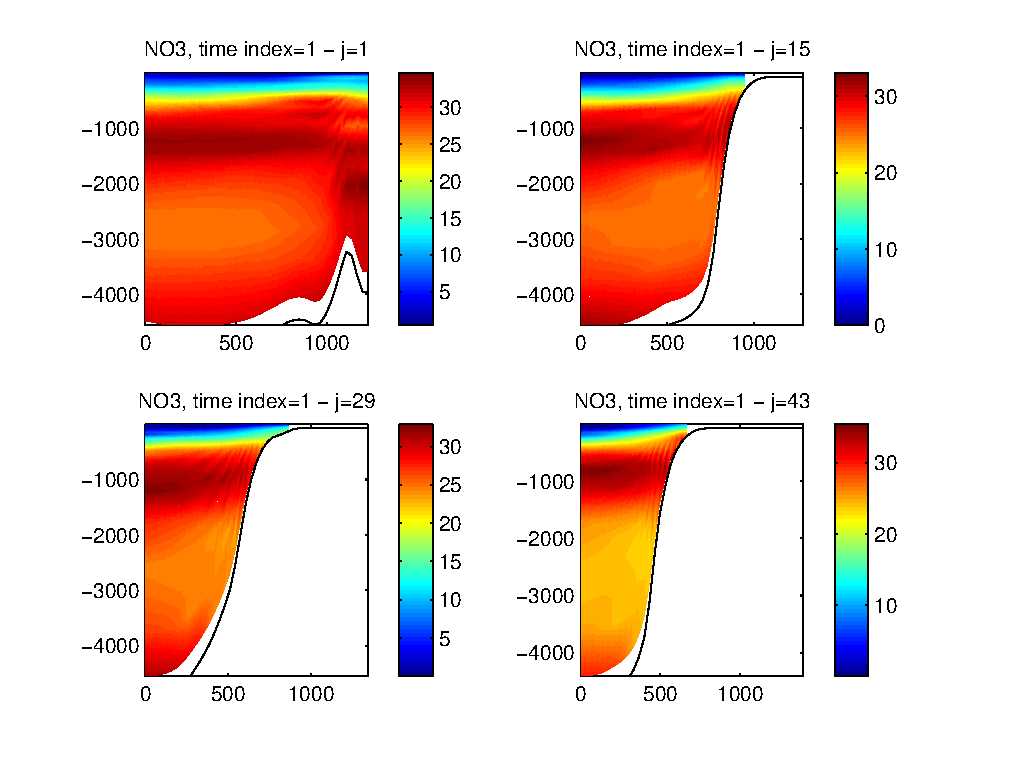
\includegraphics[width=0.70\textwidth]{NO3_profil_t1.eps}}
\caption{Result of make\_clim\_pisces for the Benguela example : NO3 forcing
  fields [mMol N m-3].}
\label{fig:makeclimpiscesNO3}
\end{figure}


\begin{figure}[!htbp]
\subfigure[Surface map]{
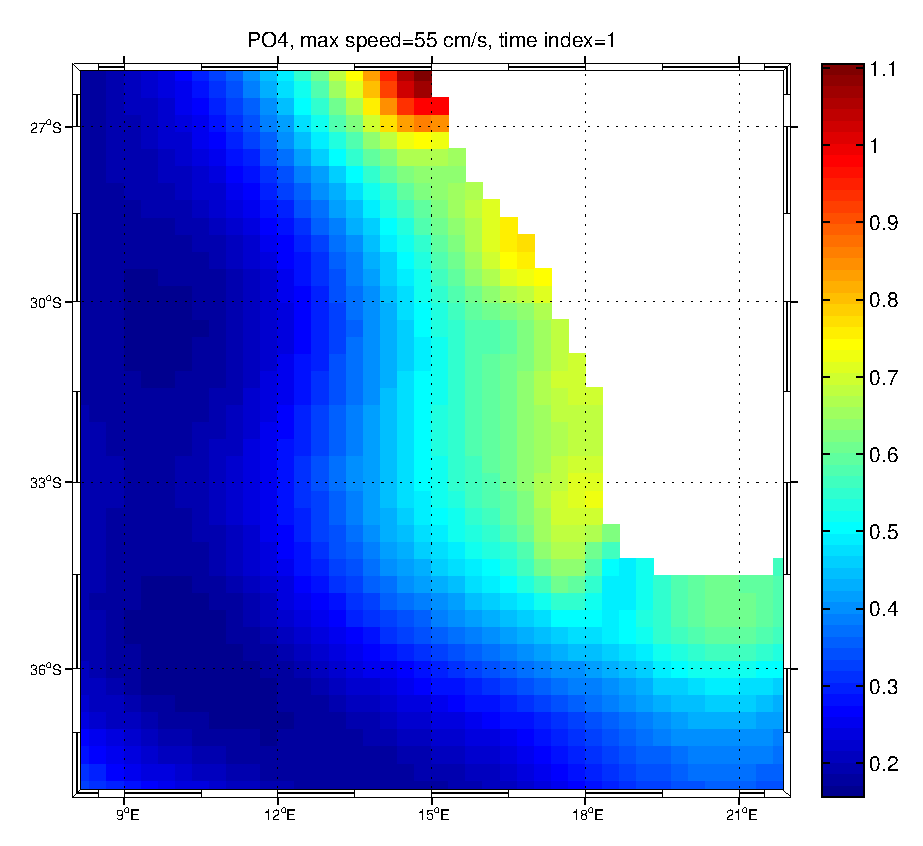
\includegraphics[width=0.4\textwidth]{PO4_surf_t1.eps}}%
\hfill
\subfigure[vertical sections along open boundaries]{
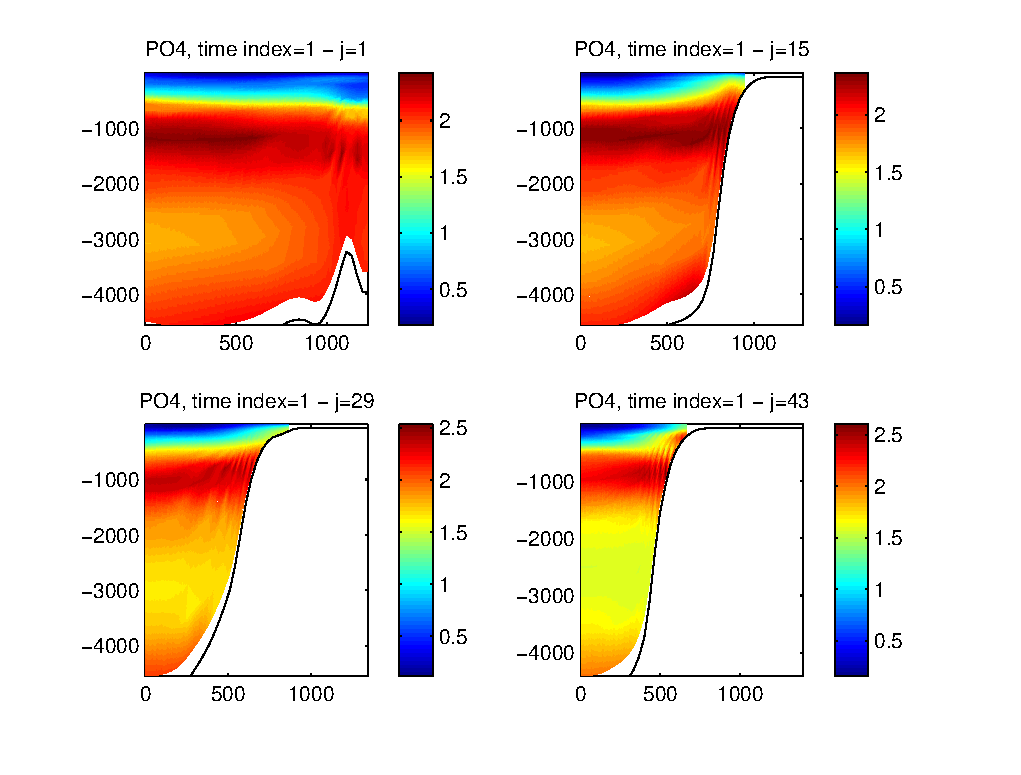
\includegraphics[width=0.70\textwidth]{PO4_profil_t1.eps}}
\caption{Result of make\_clim\_pisces for the Benguela example : PO4 forcing fields
  [mMol P m-3].}
\label{fig:makeclimpiscesNO4}
\end{figure}

\noindent To compute the Iron dust deposition forcing file xxx\_frcbio.nc file :\\
$>>$\\
$>>$ make\_dust\\
\begin{figure}[!htbp]
\centering
\subfigure{
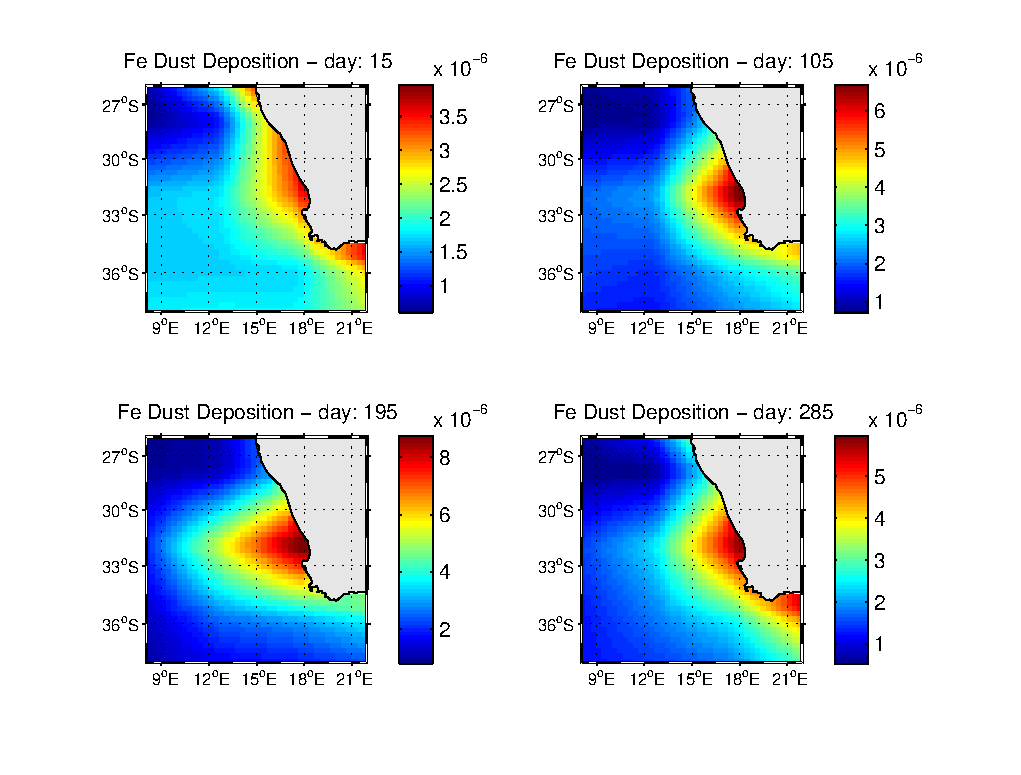
\includegraphics[width=0.8\textwidth]{dustdepo_surface.eps}}%
\hfill
\caption{Result of make\_clim\_pisces for the Benguela example : Iron dust deposition
  forcing fields [nmol Fe m-3].}
\label{fig:makeclimpiscesNO4}
\end{figure}